\documentclass[a4paper]{article}

% Includes packages relevant to Senior Lab

% character set specifications
\usepackage[english]{babel}
\usepackage[utf8]{inputenc}

% increased vertical spacing for tables
\newcommand\topVspace{\rule{0pt}{2.6ex}}      
\newcommand\bottomVspace{\rule[-1.2ex]{0pt}{0pt}} 

% extra unicode characters
\DeclareUnicodeCharacter{3BC}{\(\mu\)}
\DeclareUnicodeCharacter{3C1}{\(\rho\)}
\DeclareUnicodeCharacter{2080}{\(_0\)}
\DeclareUnicodeCharacter{2081}{\(_1\)}
\DeclareUnicodeCharacter{2082}{\(_2\)}
\DeclareUnicodeCharacter{3B5}{\(\epsilon\)}
\DeclareUnicodeCharacter{3B1}{\(\alpha\)}

% SI Units
\usepackage{siunitx}

% extra SI units
\DeclareSIUnit\gauss{G}

% enable scientific notation
\sisetup{scientific-notation = engineering, exponent-to-prefix}

% draw pretty lines
\usepackage{tikz}
\usetikzlibrary{datavisualization}
\usepackage{circuitikz}

% manual tabbing
\setlength{\parindent}{0pt}
\def\qq{\qquad}

% include graphics
\usepackage{graphicx}

% increased control over figure placement
\usepackage{float}

% box answers
\usepackage{tcolorbox}

% enable multiple section levels
\usepackage{titlesec}

% define `\subsubsubsection` command
\titleclass{\subsubsubsection}{straight}[\subsection]
\newcounter{subsubsubsection}[subsubsection]
\renewcommand\thesubsubsubsection{\thesubsubsection.\arabic{subsubsubsection}}
\titleformat{\subsubsubsection}
        {\normalfont\normalsize\bfseries}{\thesubsubsubsection}{1em}{}
\titlespacing*{\subsubsubsection}
{0pt}{3.25ex plus 1ex minus .2ex}{1.5ex plus .2ex}
\setcounter{secnumdepth}{4}

% get align environment (among other things)
\usepackage{amsmath}

% bold in math mode
\usepackage{bm}

% get \mathbb (among other things)
\usepackage{amssymb}

\usepackage{array}

% plotting
\usepackage{pgfplots}

% enable external references
\usepackage{hyperref}

% include code
\usepackage[cache=false]{minted}
\setminted{linenos, frame=lines, texcomments}

% adjust margins of individual pages (for shoving figures into place)
\usepackage{changepage}

% rotate figures
\usepackage{rotating}


\usepackage{caption}
\renewcommand{\thetable}{\arabic{section}.\arabic{table}}
\newcommand\T{\rule{0pt}{2.6ex}}       % Top strut
\newcommand\B{\rule[-1.2ex]{0pt}{0pt}} % Bottom strut

\title{PHY 4210-01 Senior Lab \\Lab P1: Planck's Constant\\Lab P6: Blackbody Radiation}

\author{Sarah Arends \\
        Jacquelyne Miksanek \\
        Ryan Wojtyla \\ \\
        Instructor: Augustus Azelis}

\date{\today}

\begin{document}
\maketitle

\begin{abstract}
%physics of experiment
%apparatus used
%what was measured
%Results
\qq 
\end{abstract}

\newpage

\tableofcontents

\newpage

P1 Planck's Constant Experiment

\newpage

\section{Objective of the Experiment}
%A brief statement on the main purpose of the experiment
\qq When demonstrating the photoelectric effect, the stopping
potential for a multitude of wavelengths is measured. The resultant
data is used to determine a value for Planck's constant through
experimentation with a photocell's cathode and a mercury lamp.

\section{Theory of the Experiment}
\qq A photon is a quantized bundle of energy that carries momentum,
but has no mass. These photons make up a general term of light. When
light comes into contact with metals, the photon energizes the atom of
the metals. If sufficient enough this energy will cause the unbound
electrons in the metal to absorb the energy and leave the metal. This
is known as the photoelectric effect. An anode can then collect the
electrons and an electrical current is the result. It is important to
note that increasing the intensity of the light will not increase the
kinetic energy of the electrons. Applying a voltage between and anode
and a cathode will exert a force toward the anode. When the voltage
is increased to the stopping potential the quantity of energy is then
equal to the kinetic energy of the electron. If the the law of
conservation of energy holds true then the kinetic energy of the
electron should be equal to the energy given to the electron by the
photon minus the energy that is transferred when the electron leaves
the metal. When the voltage exceeds the stopping potential voltage,
the photocurrent reverses and a negative current is registered on the
ammeter. The kinetic energy of light is equated to be $ E = hf$, where
$E$ is the energy, $h$ is the Planck constant, and $f$ is the
frequency. The work function of the metal is given by $W$ in the
following equation: $ W = h \times f - e \times V_0$. $V_0$ is the
stopping potential, and $e \times V_0$ is the kinetic energy. The work
function describes the quantity of energy that is necessary for a
photon to release an electron from the metal.

\section{Equipment Utilized}
%List principal pieces of apparatus used by manufacturer, model and
%serial number. When it may be important, list principal
%specifications of certain pieces of equipment (e.g. the focal length
%of an optical system, etc.)

% Description of set-up in prose
\qq A DC power supply is connected in parallel to a voltmeter. The
voltmeter will monitor the voltage of the setup and will be used to
take note of the stopping potential. A Keithley Picoammeter, and
photocell are connected in parallel to the DC power supply. The
Picoammeter will read the resultant current. A Mercury Lamp will be
placed a distance apart from the photocell, with the circular bulb
opening in alignment with the photocell's receptor window. When the
spectral filters are applied, they will be slid into the slotted grove
directly in front of the circular bulb opening on the Mercury Lamp. \\

Equipment utilized is listed below:

% List of specs
\begin{itemize}
\item Phototube 
\item Mercury Lamp 
\item Spectral Filters 
\item Daedelon Corporation Photocell 
\item DC Power Supply 
\item Keithley Picoammeter 
\item Voltmeter 
\end{itemize}

%Labeled sketch of the experimental setup
\begin{figure}[H]
\centering
% uncomment the line below to add image
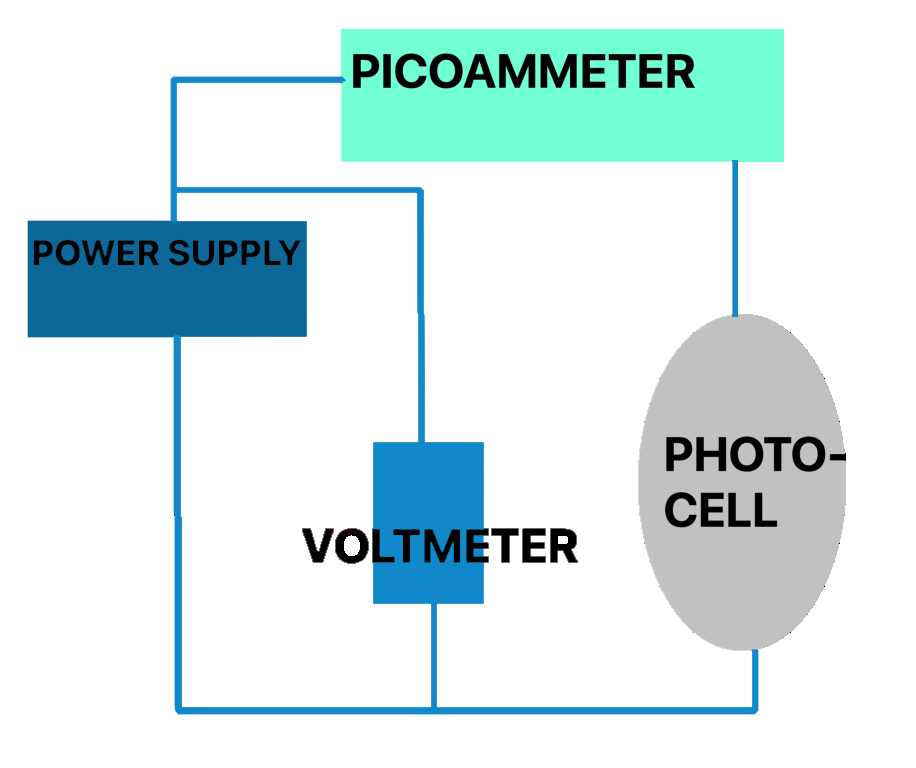
\includegraphics[width=0.75\textwidth]{photo_circuit.png}
\captionof{figure}{Circuit diagram for the photoelectric
  effect experiment}
\label{photo_circuit}
\end{figure}

\section{Procedure}

% Describe the main steps in the experimental procedures. Be sure to include any
% precautions. Sufficient details should be given such that another student can
% follow and do the experiment.

\qq The experiment begins by turning on the Mercury Lamp, a constant
level of brightness is achieved by letting the Mercury Lamp warm-up
for conservatively an hour. In the interest of time the Mercury Lamp
was warmed-up for approximately twenty minutes. Remember to have the
Mercury Lamp directed toward a wall for safety. Ensure that the
photocell's anode and cathode is connected directly to the
Picoammeter, use caution when handling the wires on the photocell as
they are fragile and fray easily. Do not allow the applied voltage to
exceed 40 volts and the current to exceed 20 $mA$. The
Picoammeter should be configured to readout the current in units of
$\mu A$. To measure the ambient background, point the photocell's
window toward the ceiling. If the experiment is to be completed with
the room lights off, then the background should be measured in the
same setting. The photocurrent of the ambient background can then be
measured to an uncertainty of $\pm$ 1 nA. The next measurement to
be taken is the unfiltered light from the Mercury Lamp. This time the
window of the photocell should be pointed toward the circular bulb
opening on the lamp, ensure that the opening is aligned with the
window. The resultant photocurrent is then recorded. The following
steps are used to measure the stopping potential for a spectra of
differing wavelengths using spectral filters. The wires to the
Picoammeter are disconnected and a DC power supply is added to the
circuit, keeping the power supply switched off. The voltage control
knob should be set to the lowest possible setting, ideally zero. The
current limit switch should be limited to 0.5 amps, and then the
current is adjusted to a moderate position within it. Turn the knob on
the photocell to its lowest setting. This is the photocell's built-in
potentiometer. The circuit can then be assembled as depicted in
\ref{photo_circuit}. Before the power supply is switched on, the
entire circuit and settings should be double-checked to ensure the
safety of the equipment. If the circuit needs to be altered it is
important to place the Picoammeter into zero-check mode (denoted by
ZCH), this is a safe mode for the ammeter to ensure it is not
overloaded. Slowly turn the voltage on the DC power supply up to 6
volts. The stopping potential should not be increasing here, this can
be monitored on the voltmeter. Slowly the resistance of the
potentiometer should be increased, and the stopping potential,
displayed on the voltmeter, should increase negatively between 0 and
-2 volts. It is important to note that while this value is becoming
more negative the current should be slowly increasing from a negative
number to zero. The stooping potential is reached when the current is
equal to zero. Record the measurements during this process, and plot
the potential versus the current. This is repeated for all of the
varying filters that accompanied the Mercury Lamp. A graph of the
potential versus the light frequency is then created. The slope of
this graph is the experimental Planck's constant value.

\subsection{Procedural Modifications}

\qq It is important to note that the potentiometer on the photocell
had a range of 0 to -1.5 volts, and thus the whole range was not
tested as it could not be. This differs from the lab manual. It is
also important to note that the stopping potential was not determined
for all filters as some had a stopping potential greater than the
absolute value of the -1.5 volt maximum of the photocell.

\subsection{Safety Tips}

\qq Please note that the Mercury Lamp emits ultra-violet light and
looking directly at the bulb can cause cataracts in the eyes. Always
ensure that the Mercury Lamp is facing a wall and is not shining on
anyone in the laboratory.


\section{Data Analysis}

%Graphs, figures, and tables with captions
%Results with error analysis
%Calculate discrepancies from theory

\qq While some filters appeared to be similar in color they were not
the same filters and every filter was indeed labeled differently. The
darker filters reduced the intensity of the light that interacts with
the photocell and does affect the stopping potential for these
filters. These darker filters have a stopping potential of a higher
absolute value, then the filters that were lighter in appearance. 

%%%%%%% NEEDS GRAPHS I_V AND I_F!

\qq The y-intercept of the graph of the voltage versus the
frequency corresponds to the stopping potential at that wavelength. 
 
%%%%%%% NEEDS PLANCK'S CONSTANT! 
%%%%%%% NEEDS PROPAGATED ERROR! 

\section{Results}

%%%%%% NEEDS SIGMA STUFF!

\subsection{Source of Error}

\qq Build-up and contaminants on certain filters causes random
intrinsic error in the measurements. The blue-grey filter labeled 160
had a residue lightly coating the surface which would absorb photons
that otherwise would not be absorbed. This would lower the absolute
value of the stopping potential as it would decrease the intensity of
the light that interacts with the photocell. The unlabeled aqua filter
had a more severe case of this as it appeared to be heavily coated
with a plaster-like substance. Once again the absolute value of the
stopping potential would decrease randomly. It is important to note
that the residues were not evenly coated on these filters. Some
filters were too big to fit in the slits on the Mercury lamp and thus
had to be held in front of the mercury bulb opening. This would be a
random intrinsic error. Errors arise if the filter is not properly
held in the same position as the filter may not be uniform or could
slip and let unfiltered light into the photocell. This could cause an
increase in the absolute value of the stopping potential, if
unfiltered light is let through. A decrease or increase in the
absolute value of the stopping potential if the filter is
non-uniform. The misalignment of the photocell window and the mercury
bulb opening would cause a systematic intrinsic error in the
measurements. The misalignment would cause a decrease in the absolute
value of the stopping potential. A non-uniformity of the Mercury Lamp
is an intrinsic systematic error that would cause the measurements to
decrease due to the decrease of the intensity of the bulb. This would
occur if the Mercury Lamp did not warm-up properly or for a long
enough time or if it is non-uniform by nature. This lab assumes an
ideal source.

\section{Conclusion}
%Brief summary, discussion of theory

\qq %%%%%%%%%%% NEEDS CONCLUSION

\newpage

P6: Blackbody Radiation

\newpage

\section{Objective of the Experiment}
%A brief statement on the main purpose of the experiment
\qq An incandescent light bulb is used in this experiment as an example of a blackbody radiator. The emission spectrum of the light bulb was measured for various temperatures. The peak wavelength of each emission spectrum was compared to a theoretical peak wavelength, derived using Wien's law and a calculated temperature of the bulb.

\section{Theory of the Experiment}

\qq Any object with nonzero temperature emits electromagnetic radiation. An idealized version of such an object is a "blackbody", which is a perfect absorber and emitter of radiation for all wavelengths. The distribution of emitted thermal energy depends only on the temperature of the blackbody. The temperature of the blackbody can be varied by changing the voltage, and therefore the intensity, of the light bulb. Thus, a series of emission spectra can be produced for a series of temperatures. When relative intensity is plotted against wavelength, a blackbody emission curve is produced that follows Planck's radiation law, given by equation \ref{eq:planck_law}, where $c$ is the speed of light, $k$ is Boltzmann's constant, $T$ is the temperature of the blackbody, and $\lambda$ is the wavelength of the electromagnetic radiation.

\begin{equation}
\label{eq:planck_law}
I \left( \lambda \right) = 
\frac{2 \pi c^2 h}{\lambda^5}
\left( \frac{1}{e^{\frac{hc}{\lambda k T} - 1}} \right)
\end{equation}

\qq The peak of this distribution is given by Wien's law, seen in equation \ref{eq:wien}. Here, the temperature $T$ is the temperature of the bulb filament. This will be calculated from the voltage and current through the bulb in the data analysis section.

\begin{equation}
\label{eq:wien}
\lambda_{max} = \frac{0.002898 \: mK}{T}
\end{equation}

\section{Equipment Utilized}
%List principal pieces of apparatus used by manufacturer, model and
%serial number. When it may be important, list principal
%specifications of certain pieces of equipment (e.g. the focal length
%of an optical system, etc.)

% Description of set-up in prose
\qq The equipment is mounted on the optics bench. The light source is fixed to one end of the bench, and a prism is oriented such that the light source is incident on its apex. The light sensor is attached to a rotating arm, mounted over a labeled disk used to determine the angle of the configuration. In front of the sensor is a collimating lens and collimating slit, separated by a distance equal to the focal length of the lens. A schematic of this experiment is shown in figure \ref{blackbody_circuit}. \\

Below is a list of some of the key pieces of equipment used in this experiment:

% List of specs
\begin{itemize}
\item Optics bench, used to mount equipment
\item Prism spectrophotometer kit, including collimating slits
\item Broad spectrum light sensor
\item Pasco Capstone software for data acquisition
\item Multimeters, for current and voltage measurements
\end{itemize}

%Labeled sketch of the experimental setup
\begin{figure}[H]
\centering
% uncomment the line below to add image
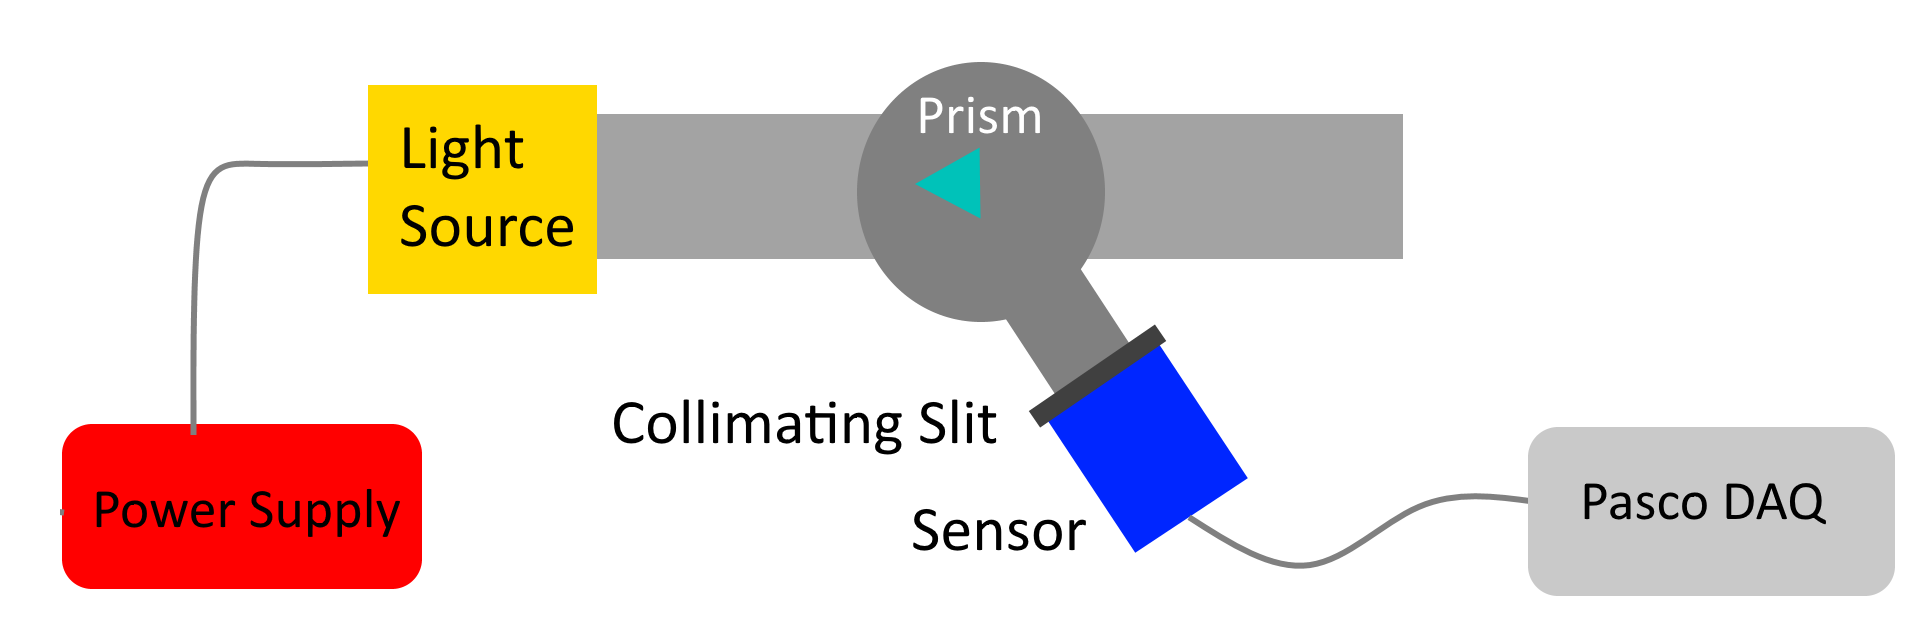
\includegraphics[width=\textwidth]{blackbody_circuit.png}
\captionof{figure}{Circuit diagram for the blackbody radiation experiment}
\label{blackbody_circuit}
\end{figure}

\section{Procedure}
% Describe the main steps in the experimental procedures. Be sure to include any
% precautions. Sufficient details should be given such that another student can
% follow and do the experiment.

\qq By having the "blackbody" light source incident on the prism, this set-up allows the entire spectrum to be measured without running into issues caused by diffraction grating. Based on the geometry of the prism, Snell's law will be used to determine the index of refraction, and therefore the wavelength of the incident light (discussed further in the data analysis section). For each incident angle, the corresponding relative intensity is measured with a spectrophotometer, connected to the Pasco Capstone data acquisition software. The spectrophotometer is grounded to the power supply being used to power the light bulb. Two multimeters are used to monitor the current and voltage of the light bulb. The applied voltage was limited to 10 volts to avoid damaging the bulb. The angle was changed in increments of one degree in order to scan through the resultant emission spectrum.

\subsection{Procedural Modifications}
\qq 

\section{Data Analysis}
%Graphs, figures, and tables with captions
%Results with error analysis
%Calculate discrepancies from theory

\qq As the temperature of the light bulb is lowered, the peak of the blackbody curve shifts towards [HIGHER/LOWER] wavelength. Equation \ref{eq:wien} predicts that a lower temperature corresponds to a peak in the longer/greater wavelength spectrum, since the wavelength is inversely proportional to the temperature. Experimental data indicated that as temperature of the light bulb was lowered, the overall intensity of the distribution [INCREASES/DECREASES]. Planck's radiation law also theorizes that decreasing temperature corresponds to decreasing intensity, since the two quantitites are directly proportional.

\qq The temperature of the light bulb filament must be calculated from the measured voltage and current for each trial. The resistance of the filament is first determined using a modified form of Ohm's law, $R=V/I$. Resistivity, $r$, can be calculated from this resistance using equation \ref{eq:resistivity}, where $r_0 = 5.65 \mu \Omega cm$ is the resistivity of Tungsten at room temperature, $R_{bulb}=0.93 \Omega$ is the resistance of the bulb, and $V/I$ is the calculated resistance of the filament. 

\begin{equation}
\label{eq:resistivity}
r =
\left(
\frac{\frac{V}{I}-0.2}{R_{bulb}}
\right)
\end{equation}

A sample calculation is shown below for the case of an applied voltage of $3V$:
\begin{align*}
r &=
\left(
\frac{\frac{3}{0.388}-0.2}{0.93}
\right) \\
&= 45.8 \; \mu \Omega cm
\end{align*}

Temperature was calculated from resistivity using the following fit equation:
$$T[K] = 103 + 38.1r - 0.095r^2 = (2.48\times 10^{-4}) r^3$$
For the $3V$ case discusses above, for example, the temperature was determined to be $1671K$. From the temperature of the filament, Wien's law is used to determine a theoretical value of $\lambda_{peak}$. This information is summarized in table \ref{table:temps}.

\begin{center}
\begin{tabular}{|c|c|c|}
\hline 
Voltage & Temperature & Theoretical $\lambda_{peak}$ \topVspace \bottomVspace \\
\hline
3V & 1671 K & $1.73 \times 10^{-6}$ m \\
5V & 2031 K & $1.43 \times 10^{-6}$ m\\
7V & 2317 K & $1.25 \times 10^{-6}$ m\\
9V & 2540 K & $1.14 \times 10^{-6}$ m\\
\hline
\end{tabular}
\label{table:temps}
\captionof{table}{Calculated temperature of light bulb filament for each applied voltage; this is used to determine theoretical peak wavelength}
\end{center}

DO THESE WAVELENGTHS COINCIDE WITH THE PEAKS ON OUR GRAPHS?

\qq Substituting the sun's temperature into Wien's law, it is determined that the peak wavelength is around 500nm, which is in the green spectrum of visible light. However, sun clearly does not appear green. This is because the emission spectrum is a continuum throughout the visible light region, and the colors will combine to appear white to an observer.

\qq The highest temperature tested was 2540 K, associated with a voltage of 9 V. For this temperature, more of the intensity is in the [VISIBLE/INFRARED] portion of the spectrum. If the goal of the light bulb is to produce the most light for a given voltage, the intensity should peak in the visible light spectrum. To move the portion of the spectrum in the infrared region to the visible region, the temperature can be increased to shift the distribution to lower wavelengths.

\section{Results}

\qq For each of the four voltages, the relative intensity of light incident upon
the broad spectrum light sensor was plotted against the wavelength of the light
being measured by the sensor.

\qq First, \SI{3}{\volt} and \SI{0.388}{\ampere} were applied to the
bulb. Although no clear pattern can be readily discerned from the plot, Figure
\ref{gph:3volt}, at lower wavelengths, a clear peak of intensity occurs at
\( 939 \pm 1 \si{\nano\meter} \). This value is within the range of the
theoretical peak wavelength of \( 1734 \pm 1292 \si{\nano\meter} \). 

\begin{figure}[H]
  \begin{center}
    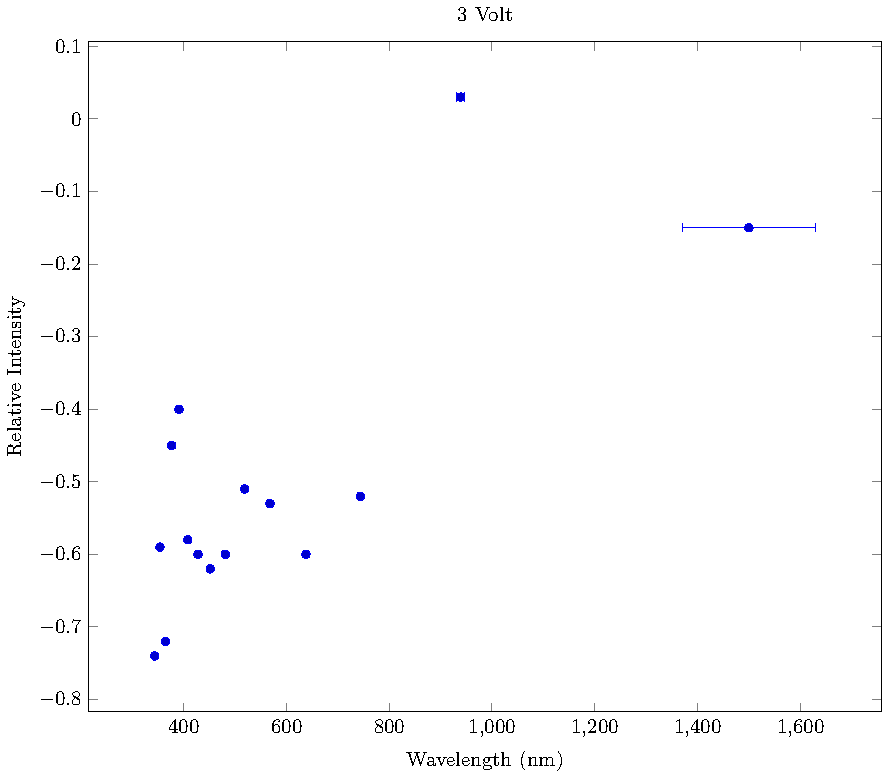
\includegraphics[width=0.5\textwidth]{P6-BlackbodyRadiation/Plots/3Volt/3volt.pdf}
  \end{center}
  \label{gph:3volt}
  \caption{The relative intensity was plotted against the wavelengths in order
    to find the peak wavelength.}
\end{figure}

\qq The discrepancy between the theoretical and experimental values of the peak
wavelength is calculated with
\( \Delta_{\lambda} = | \lambda_t - \lambda_e | \), where \( d \) is the
discrepancy, \( \lambda_t = 939 \pm 1 \si{\nano\meter} \) is the theoretical
value of the peak wavelength, and
\( \lambda_e = 1734 \pm 1292 \si{\nano\meter} \) is the experimental value of
the peak wavelength.

\begin{align*}
  \Delta_{\lambda} =& \left| (939) - (1734) \right| \\
  \Delta_{\lambda} =& 795 \si{\nano\meter} \\
\end{align*}

Since the standard deviation of the wavelengths at \SI{3}{\volt} is \(
\sigma_{\lambda} = \SI{306}{\nano\meter} \), the experimental value of \(
\lambda_e = 1734 \pm 1292 \si{\nano\meter} \) at \SI{3}{\volt} is

\begin{equation*}
  \frac{\Delta_{\lambda}}{\sigma_{\lambda}} = \frac{795}{306} = 2.60 \sigma
\end{equation*}

from the theoretical value of \( \lambda_t = 939 \pm 1 \si{\nano\meter} \).

\qq 

\subsection{Source of Error}

\section{Conclusion}
%Brief summary, discussion of theory

\section{Appendices}

\end{document}
